
\documentclass[12pt, a4paper, oneside, english, Computer Modern Roman]{teza-upb}
\setcounter{secnumdepth}{3}
\setcounter{tocdepth}{3}

\usepackage{babel}
\usepackage{color}
\usepackage{graphicx}
\graphicspath{  {C:/Users/tudor_ytmdyrk/Desktop/pozeLicenta/}  }
\usepackage[
  bookmarks,
  bookmarksopen=true,
  pdftitle={Dizertatie},
  linktocpage]{hyperref}


\singlespacing


%%%%%%%%%%%%%%%%%%%%%%%%%%%%%%%%%%%%%%%%%%%%%%%%%%%%%%%%cod colorat
\usepackage{listings}
\usepackage{color}
 
\definecolor{codegreen}{rgb}{0,0.6,0}
\definecolor{codegray}{rgb}{0.5,0.5,0.5}
\definecolor{codepurple}{rgb}{0.58,0,0.82}
\definecolor{backcolour}{rgb}{0.95,0.95,0.92}

\lstdefinestyle{mystyle}{
	language=Matlab,
 %   backgroundcolor=\color{backcolour},   
    commentstyle=\color{codegreen},
    keywordstyle=\color{blue},
    numberstyle=\tiny\color{codegray},
    stringstyle=\color{codepurple},
	basicstyle=\ttfamily\scriptsize,
    breakatwhitespace=false,         
    breaklines=true,                 
    captionpos=b,                    
    keepspaces=true,                 
    numbers=left,                    
    numbersep=5pt,                  
    showspaces=false,                
    showstringspaces=false,
    showtabs=false,                  
    tabsize=2
}
 
\lstset{style=mystyle}
%%%%%%%%%%%%%%%%%%%%%%%%%%%%%%%%%%%%%%%%%%%%%%%

\begin{document}

\author{Predună Tudor-Gabriel}

\title{Basmele românilor}


\facultatea{Facultatea de Electronică, Telecomunicații și Tehnologia Informației}
\tiplucrare{licență}
%\tiplucrare{dizertație}
\domeniu{Electronică, Telecomunicații și Tehnologia Informației}
\catedra{Telecomunicații}
\campus{Leu} 
\program{Povești}
\titlulobtinut{Inginer}

\director{Iulian Năstac} 

\submissionmonth{Iunie} 
\submissionyear{2022} 







\chapter{Connecting to the Pulse Oximeter}



\begin{figure}[h]
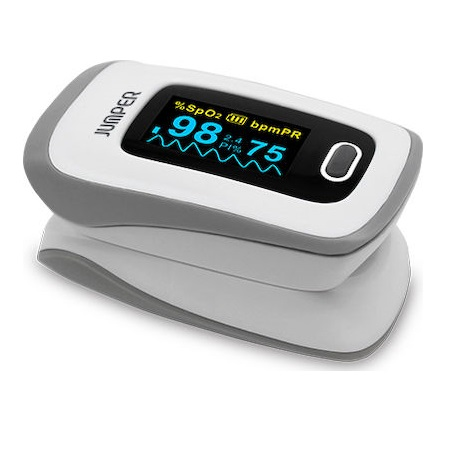
\includegraphics[scale=1]{jumper}
\end{figure}




\end{document}

